\documentclass{article}

\usepackage[version=3]{mhchem}
\usepackage[greek,english]{babel}
\usepackage{booktabs}
\usepackage{gensymb}
\usepackage{graphicx}
\usepackage[hidelinks]{hyperref}
\usepackage{fixltx2e}
\usepackage{titlesec}
\usepackage[normalem]{ulem}
\usepackage{parskip}
\usepackage{multirow}
\usepackage{fancyvrb}
\usepackage{color}
\usepackage{float}
\usepackage[super]{nth}
\usepackage{minted}
\usepackage{etoolbox}

\titleformat*{\section}{\Large\bfseries}
\titleformat*{\subsection}{\bfseries}

\hypersetup{
  colorlinks   = true,
  urlcolor     = blue,
  linkcolor    = black,
  citecolor    = black
}

\definecolor{grey}{gray}{0.65}

\newfloat{listing}{thp}{lop}
\floatname{listing}{Listing}

% Use the Borland theme for code samples, but don't italicize comments.
\usemintedstyle{borland}
\AtBeginEnvironment{minted}{\let\itshape\relax}

\setcounter{secnumdepth}{0}

\newcommand{\calpha}{C\textsubscript{\textgreek{a}}}
\newcommand{\ahelices}{\textgreek{a}-helices}
\newcommand{\bsheets}{\textgreek{b}-sheets}
\newcommand{\bbphi}{\ensuremath{\phi}}
\newcommand{\bbpsi}{\ensuremath{\psi}}
\newcommand{\bbomega}{\ensuremath{\omega}}
\newcommand{\module}[2]{\href{#2}{\texttt{#1}}}
\newcommand{\atomrec}{\texttt{ATOM} record}

\newenvironment{lpthw}
{Relevant LPTHW:}
{}

\newenvironment{problems}
{\subsubsection{Before moving on...} \begin{enumerate}}
{\end{enumerate}}

\begin{document}

\title{Making Ramachandran Plots}
\author{Bootcamp Summer Programming Project}
\date{}
\maketitle{}

\section{Introduction}

The purpose of this project is to give you some practice using Python in a 
scientific context.  We designed the project for beginning programmers, but 
before starting you'll still have to teach yourself the basics of Python.  We 
recommend the book \emph{Learn Python the Hard Way} (LPTHW), which you can 
either \href{http://learnpythonthehardway.org/book/}{read for free online} or 
\href{https://paydiv.io/access/buy/2/}{purchase}.

The project is to write a program that generates Ramachandran plots from 
\href{http://www.rcsb.org/pdb/home/home.do}{Protein Data Bank} (PDB) files.  
Ramachandran plots show how backbone torsion angles are distributed in 
proteins.  Different features of proteins (namely \ahelices{} and \bsheets{}) 
occupy distinct regions in these plots.  For this reason, Ramachandran plots 
are commonly used both to validate experimental structures and to predict 
computational structures.

The project is divided into four parts:

\begin{enumerate}
 \item Setting up Python and reading the command line.
 \item Parsing groups of four backbone atoms from PDB files.
 \item Calculating torsions angles from those groups of atoms.
 \item Plotting those torsion angles using matplotlib.
\end{enumerate}

Try to get through at least one part every two weeks.  It takes time to get 
comfortable writing code, and you won't get there if you put off the whole 
project until just before bootcamp starts.  The project will be due on the 
first day of bootcamp.  We will wrap up the project with an activity where 
everyone explains their code to a partner (i.e. a code review).  This activity 
won't be as valuable for you if you don't finish the project on time.  If you 
are worried about finishing the project on time, or have any questions about 
the project or programming in general, please don't hesitate to email any one 
of us.

\subsection{What if you already know how to program?}

Even if you already know how to program, it's still important for you to work 
through this project so that you can participate in the code review we'll be 
holding on the first day of bootcamp (see above).  In fact, you should make an 
extra effort to make your code as clean and understandable as possible so that it 
can be an example for the more novice programmers in your class.

If you know how to program, but not in Python, take this opportunity to learn 
Python.  The challenges in the \emph{Future Directions} section will be 
especially useful to you, because they will make you think a little bit more 
and really explore the language.

\section{What is a Ramachandran Plot?}

Let's begin with some basic terminology: proteins are chains of amino acid 
residues.  Figure~\ref{fig:three-residues} shows three residues from a larger 
protein.  A distinction is made between the backbone (blue) and the sidechains 
(red).  Every residue in the protein is connected through the backbone, which 
has a very regular pattern of atoms: \ce{N - C_{\textgreek{a}} - C - N - 
C_{\textgreek{a}} - C - \ldots} where the carbon that supports the sidechain is 
called \calpha{} to distinguish it from the one that doesn't.

\begin{figure}[h]
 \centering
 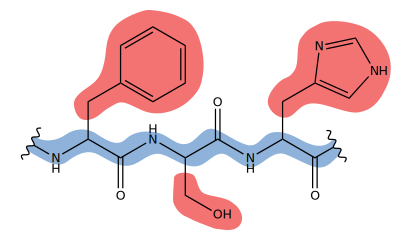
\includegraphics[width=0.60\textwidth]{three-residues}
 \caption{Three residues with the backbone and sidechains highlighted.}
 \label{fig:three-residues}
\end{figure}

Torsion angles are a convenient way to describe the geometry of the backbone.  
A torsion angle can be intuitively described as the amount of twist around a 
bond.  To be more precise, consider four consecutive backbone atoms.  You 
always need four atoms to define a torsion angle.  Use the first three atoms to 
construct one plane and the last three atoms to construct another.  The angle 
between those two planes is the torsion angle, or the twist around the bond 
connecting the second and third atoms.  These angles are a convenient way to 
describe geometry because they don't depend on the orientation of whole protein 
in Cartesian space.

For each residue in a protein, three backbone torsions are defined:

\begin{table}[h]
\centering
\begin{tabular}{cc}
\toprule
Torsion      & Backbone Atoms                                               \\
\midrule
$\omega{}_i$ & \ce{
C^{$i$-1}_{\textgreek{a}} - C^{$i$-1} - N^{$i$} - C^{$i$}_{\textgreek{a}}}  \\
$\phi{}_i$ & \ce{
C^{$i$-1} - N^{$i$} - C^{$i$}_{\textgreek{a}} - C^{$i$}}                    \\
$\psi{}_i$ & \ce{
N^{$i$} - C^{$i$}_{\textgreek{a}} - C^{$i$} - N^{$i+1$}}                    \\
\bottomrule
\end{tabular}
\caption{Backbone torsion angles.}
\label{tab:backbone-torsions}
\end{table}

A Ramachandran plot is a scatter plot showing the \bbphi{} and \bbpsi{} angles 
for each residue.  The \bbphi{} angles are plotted along the x-axis and the 
\bbpsi{} angles are plotted along the y-axis.  Each point is the $\phi_i, 
\psi_i$ pair for one residue.  The \bbomega{} angles are left out because they 
never deviate much from 180\degree.  

Figure~\ref{fig:example-plot} shows the Ramachandran plot for chain A of PDB 
ID: 1AXC, which is one of the structures we uploaded for you to use.  Note that 
there are two distinct clusters of points.  These represent two specific 
backbone conformations that are common in folded proteins: \ahelices{} (lower 
cluster) and \bsheets{} (upper cluster).  The ability to easily identify which 
residues are contributing to well-known, stable structural motifs is what makes 
Ramachandran plots useful for structural validation and prediction. 

\begin{figure}[h]
 \centering
 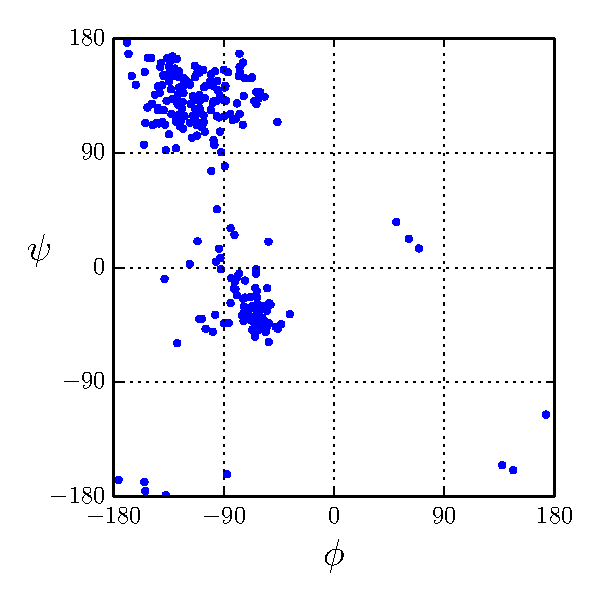
\includegraphics[width=0.45\textwidth]{example-plot}
 \caption{Ramachardran plot for chain A of PDB ID: 1AXC}
 \label{fig:example-plot}
\end{figure}

\section{What Do You Need to Do?}

Your task is to create a program written in Python that takes a PDB file 
(specified on the command line) as input and produces a Ramachandran plot as 
output.  Use the paragraphs below to guide how you write your  program.  You 
can download some example inputs from the
\href{http://bootcamp.ipqb.org/programming}{bootcamp website}.

\subsection{Part 1: Using Command Line Arguments}

\begin{lpthw}
Through Exercise 13.
\end{lpthw}

Before anything else, you need to install Python on your computer and learn how 
to run a ``Hello world!" program.  Exercises 0 and 1 of LPTHW explain how to do 
this pretty well for a variety of systems, but if you get stuck email one of us 
and we'll make sure you can get started.  Once you've done this, read as much 
of LPTHW as you can.  If you're learning how to program for the first time, we 
recommend that you take notes as you work through the exercises.

Your program should accept the name of a PDB file as a command line argument.  
This will allow you to easily generate Ramachandran plots for different 
structures without having to change your script itself.  Exercise 13 of LPTHW 
explains how to get write programs that accept command line arguments.

\begin{problems}
 \item Write a program that just prints the name of a file specified on the 
  command line.  For example:

  \texttt{\$ python rama.py 1AXC.pdb \\ 1AXC.pdb}

  Here the \texttt{\$} sign represents the shell prompt.  The rest of that 
  first line is what you should type into the terminal to run your program.  
  The second line is the output that your program should produce.
\end{problems}

\subsection{Part 2: Reading PDB Files}

\begin{lpthw}
Through Exercise 32.
\end{lpthw}

PDB files contain information about the 3D structure of proteins.  PDB stands 
for Protein Data Bank, which is an online database of protein structures.  
These files are regular text files (so you can view them with the same program 
you use to edit Python code) where each line contains different information 
about the structure.  The lines containing the information relevant to this 
project all begin with the keyword \texttt{ATOM}:

\begin{listing}[h]
\centering
\begin{BVerbatim}[fontsize=\footnotesize,commandchars=\\\{\}]
\textcolor{grey}{         1         2         3         4         5         6         7         8}
\textcolor{grey}{12345678901234567890123456789012345678901234567890123456789012345678901234567890}
ATOM   2305  CA  ILE A 255      35.578   9.357   5.792  1.00 43.22           C  
\end{BVerbatim}
\caption{An example \atomrec{}.}
\label{list:pdb-example}
\end{listing}

Listing~\ref{list:pdb-example} shows an example \atomrec{}.  (The gray numbers 
aren't part of the record; they're just numbering the columns.)  Each 
\atomrec{} identifies a particular atom and specifies its coordinates.  
Different pieces of information about the atom are given at different offsets 
from the beginning of the line.  For example, the \nth{13}~-~\nth{16} 
characters of our example (\texttt{CA}) specify that the atom in question is a 
\calpha{}.  The \nth{18}~-~\nth{20} characters (\texttt{ILE}) specify that the 
atom is part of an isoleucine residue.
Table~\ref{tab:pdb-atom-record} describes the \atomrec{} fields that are most 
relevant to this project.  The complete 
\href{http://www.wwpdb.org/documentation/format33/v3.3.html}{PDB file format} 
is also available online if you're interested.

\begin{table}[h]
\centering
\begin{tabular}{r@{ - }lcll}
\toprule
\multicolumn{3}{l}{Columns} & Example         & Description                         \\
\midrule
 1 &  6 & & \texttt{ATOM}   & Record type                         \\
 7 & 11 & & \texttt{7507}   & Atom serial number                  \\
13 & 16 & & \texttt{CA}     & Atom name                           \\
18 & 20 & & \texttt{ILE}    & Residue name                        \\
23 & 26 & & \texttt{255}    & Residue sequence number             \\
31 & 38 & & \texttt{35.578} & X coordinate of atom                \\
39 & 46 & & \texttt{9.357}  & Y coordinate of atom                \\
47 & 54 & & \texttt{5.792}  & Z coordinate of atom                \\
\bottomrule
\end{tabular}
\caption{Description of the fields in an \texttt{ATOM} record.}
\label{tab:pdb-atom-record}
\end{table}

Learning how to break big problems into smaller problems is an important skill 
for new programmers to practice.  This part of the project is a good place to 
do so because there are lots of ways to take small steps and get intermediate 
results when parsing a file.  The milestones listed below break down some of 
your first steps, but they may still be challenging.  If you get stuck, think 
about ways to break down the problem even further.

This is also a good time to focus on writing good comments.  A good rule of 
thumb is that you should have a comment describing anything you needed to look 
up when writing the code in the first place, because when reading the code 
months from now, those are probably the things that will confuse you the most.  
Remember, we'll be going over this project on the first day of bootcamp.  
You'll get more out of that session if you can remember why you wrote your 
program the way you did.

\begin{problems}
 \item Print out all the lines in the PDB specified on the command line.

 \item Extract the $x$, $y$, and $z$ coordinates for each atom in the PDB file.

 \item To calculate each \bbphi{} and \bbpsi{} torsion, you need coordinates 
  for four atoms.  Table~\ref{tab:backbone-torsions} shows which coordinates 
  are needed for which torsion.  Make groups of all the coordinates you'll need 
  to calculate each torsion angle.
\end{problems}

\subsection{Part 3: Calculating Torsion Angles}

\begin{lpthw}
Exercises 18-21.
\end{lpthw}

Once you've read in Cartesian coordinates for all the backbone atoms, you'll 
need to calculate torsion angles.  You can find the algorithm for this 
calculation 
\href{http://math.stackexchange.com/questions/47059/how-do-i-calculate-a-dihedral-angle-given-cartesian-coordinates}{here}.  
Notice that this algorithm involves a healthy dose of vector arithmetic.  Since 
Python doesn't have built-in support for vector arithmetic, you'll have to 
write and test your own functions to perform the tasks outlined in 
Table~\ref{tab:vector-functions}.  Listing~\ref{lst:example-function} shows 
what one of these functions might look like.  Keep in mind that a vector is 
nothing more than a set of three coordinates, like the tuples we used above to 
store the backbone atom coordinates.  

\begin{table}[h]
\centering
\begin{tabular}{lll}
\toprule
Function                  & Example Input                & Example Output              \\
\midrule
Add two vectors           &
 \texttt{(1, 2, 3) (3, 4, 5)} & \texttt{(4, 6, 8)}          \\
Subtract two vectors      &
 \texttt{(1, 2, 3) (3, 4, 5)} & \texttt{(-2, -2, -2)}       \\
Normalize a vector        &
 \texttt{(1, 2, 3)}           & \texttt{(0.27, 0.53, 0.80)} \\
Calculate a dot product   &
 \texttt{(1, 2, 3) (3, 4, 5)} & \texttt{26}                 \\
Calculate a cross product &
 \texttt{(1, 2, 3) (3, 4, 5)} & \texttt{(-2, 4, -2)}        \\
\bottomrule
\end{tabular}
\caption{Vector arithmetic functions.}
\label{tab:vector-functions}
\end{table}

\begin{listing}[h]
 \inputminted{python}{example-function.py}
 \caption{Example addition function.}
 \label{lst:example-function}
\end{listing}

Once you have written these functions, use them to create another function that 
calculates a torsion angle using the algorithm linked above.  This function 
should take four vectors as input and return a single angle as output.  

\begin{problems}
 \item Write and test the functions listed in Table \ref{tab:vector-functions}.
 \item Write and test a function that calculates the torsion angles using the 
  algorithm linked above.  This function should accept four tuples of three 
  floats each and should return a single float.
 \item Create two lists: one that contains all the \bbphi{} torsions and one 
  that contains all the \bbpsi{} torsions.  This should build on the two loops 
  you wrote at the end of the previous section.
\end{problems}

\subsection{Part 4: Making Plots}

\begin{lpthw}
Through Exercise 40.
\end{lpthw}

Use \module{matplotlib}{http://matplotlib.org/users/pyplot_tutorial.html} to 
generate your Ramachandran plot.  LPTHW doesn't cover \texttt{matplotlib}, so 
you'll have to figure out how to install it and use it on your own.  Here are 
the official \href{http://matplotlib.org/users/installing.html} {installation 
instructions} and here is a pretty good
\href{http://matplotlib.org/users/pyplot_tutorial.html}{tutorial} that shows 
how to do the kind of things you'll need for this project.  Again, please don't 
hesitate to email one of us if you get stuck on any of this.

\section{Future Directions}

If you found this project to be useful and you want to continue improving your 
scientific programming skills, try one or more of these extra challenges:

\subsection{1. Plot interesting subsets of residues}

It can be informative to make Ramachandran plots for subsets of the residues in 
proteins.  For example, glycines and residues that come just before prolines 
(i.e. pre-prolines) have very characteristic Ramachandran plots.  Modify your 
program to either show just glycines, just pre-prolines, or everything except 
glycines and pre-prolines.  There won't be enough residues in a single 
structure to really show what these plots should look like, so try combining 
this with the challenge below to fill in your plots.  Also, if you don't 
already know, you might find it interesting to ponder why glycines and 
pre-prolines have distinctive plots.

\subsection{2. Use NumPy to speed up the vector arithmetic}

\href{http://www.numpy.org/}{NumPy} is a fast and comprehensive Python module for performing vector and matrix
calculations. Not only can using NumPy greatly simplify your code, but it also
can drastically speed it up. Also, most scientific computing and visualization packages
in Python are NumPy-compatible out of the box. Try using NumPy arrays instead of tuples
to store your vectors, and then use NumPy functions for the vector math. There are
plenty of introductory NumPy tutorials on the web. The resulting speed-ups will help
with the next future direction.

\subsection{3. Make a combined plot for 10,000 structures}

Working with lots of data is an important skill for scientific programmers.  
Toward that end, we uploaded a 
\href{ftp://ftp.biochem.ucl.ac.uk/pub/cath/v3_5_0/CathDomainPdb.S35.v3.5.0.tgz}{subset 
of the CATH database} comprising 11,926 PDB files to the bootcamp website.  
Download this data and modify your program to create a single Ramachandran plot 
for all of it.  Experiment with ways to quickly process so many files and to 
clearly present so many data points.

\subsection{4. Automatically download PDB files}

One of the nice things about Python is that it's not just for scientific 
programming, so there are libraries for doing things like downloading files 
from the web.  The PDB in particular makes it very easy to 
\href{http://www.rcsb.org/pdb/software/rest.do#search}{automatically download 
structures}.  Modify your program to accept a PDB ID rather than an actual 
file, then download that structure from the PDB and use it to generate the 
plot.  The \module{requests}{http://docs.python-requests.org} library is a good 
place to start.

\end{document}
